\documentclass[a4paper,12pt]{article}

\usepackage[top=2.5cm, bottom=2.5cm, left=3.175cm, right=3.175cm]{geometry}
\usepackage{polski}
\usepackage[utf8]{inputenc}
\usepackage{xcolor}
\usepackage{graphicx}
\usepackage{titlesec}
\usepackage{indentfirst}
\usepackage{amsmath}
\usepackage{float}
\usepackage{minted}
\usepackage[section]{placeins}
\usepackage{subfig}

% \usetikzlibrary{positioning}

\graphicspath{{images/}}

\numberwithin{equation}{section}

\newminted{cpp}{breaklines,linenos,frame=single}

\usepackage[pdftex,
            pdfauthor={Cezary Bober, Michał Kruczek},
            pdftitle={Dokumentacja projektu z przedmiotu Grafika Komputerowa},
            pdfsubject={Microcar Flex Furgon}]{hyperref}

\begin{document}

\pagenumbering{gobble}

\begin{titlepage}
    \includegraphics[height=1.75cm]{prz_pl.png}
    \hfill
    \includegraphics[height=1.75cm]{weii_pl.png}
    
    \centering
    \vfill
    
    {\Huge \textbf{Dokumentacja projektu z przedmiotu Grafika Komputerowa} \par}
	\vspace{1.5cm}
	{\LARGE Microcar Flex Furgon \par}
	
	\vfill
    
    {\Large \textbf{Cezary Bober} \par}
    {\Large \textbf{Michał Kruczek} \par}
    
    \vfill
    
    {\LARGE Rzeszów, 2019\par}
\end{titlepage}

\setlength{\parskip}{0.3cm}
\setlength{\parindent}{1cm}
\pagenumbering{arabic}
\setcounter{page}{2}

\tableofcontents
\pagebreak

\section{Opis projektu}
Celem projektu było stworzenie interaktywnego modelu prostego samochodu korzystając z biblioteki OpenGL. Dzięki wykonaniu projektu poszerzyliśmy naszą wiedzę dotyczącą zarówno tworzenia modeli 3D jak i z pozostałych zagadnień składających się na dziedzinę jaką jest grafika komputerowa. 

Stworzony pojazd z pozwala na jazdę do przodu oraz do tyłu, zaimplementowane zostały także pewne elementy interaktywne takie jak otwieranie i zamykanie klapy bagażnika oraz maski. Samochód posiada także kręcący się wał napędowy napędzający potężny silnik.

\subsection{Wykorzystane technologie}
Projekt został napisany przy wykorzystaniu języka C++ w wersji 11. Przy tworzeniu projektu wykorzystywaliśmy bibliotekę graficzną \textit{OpenGL}. Oprócz niej wykorzystana została biblioteka \textit{OpenGL Mathematics}, która pozwala na proste wykorzystanie bardziej skomplikowanych narzędzi aparatu matematycznego. Kolejną biblioteką była \textit{GLFW}, która zapewnia proste API do tworzenia okien, kontekstów i powierzchni, odbierania danych wejściowych i zdarzeń. Załadowanie tych bibliotek było możliwe dzięki bibliotece \textit{OpenGL Extension Wrangler Library}, która zapewnia wydajne mechanizmy uruchamiania w celu określenia, które rozszerzenia OpenGL są obsługiwane na platformie docelowej.

Modele poszczególnych części samochodu zostały stworrzone w narzędziu \textit{Blender}, który jest otwartym oprogramowaniem do modelowania i renderowania obrazów oraz animacji trójwymiarowych. Następnie dzięki bibliotece \textit{Open Asset Import Library} zostały one umieszczone w programie.


\section{Inspiracja}
Inspiracją do stworzenia omawianego modelu samochodu był posiadany przez jednego z autorów projektu samochód \textit{Microcar MC1} przedstawiony na zdjęciu poniżej.
\begin{figure}[h!]
    \centering
    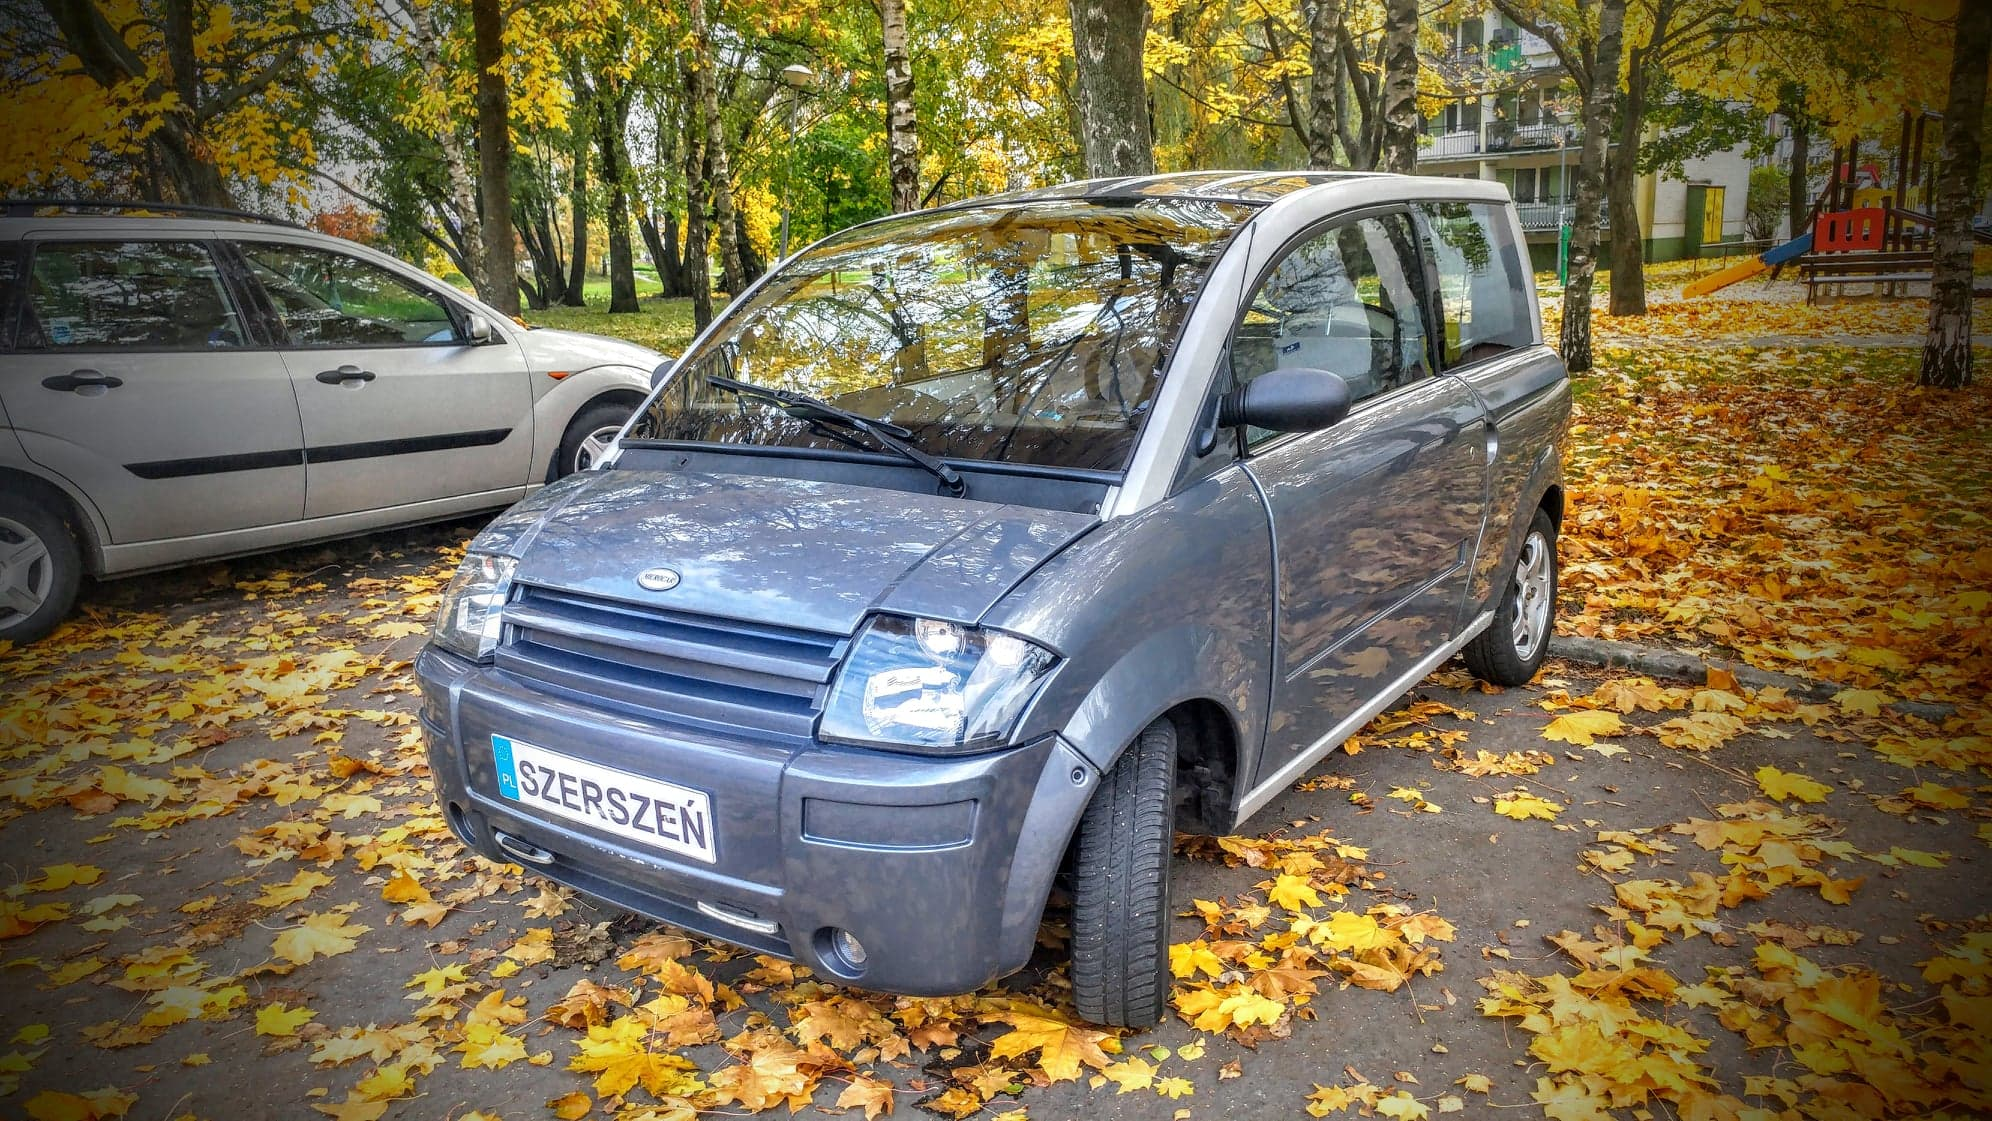
\includegraphics[width=\textwidth]{szerszen.jpg}
    \caption{Microcar MC1 \textit{"Szerszeń"}}
    \label{fig:szerszen}
    \vspace{1cm}
\end{figure}

Umieszczona w projekcie wersja jest modelem zmodyfikowanym na potrzeby handlu towarowego. Niewielkie rozmiary i mała waga powodują, że jest to bardzo dobry pojazd do ciasnych i zatłoczonych miast.
\begin{figure}[h!]
    \centering
    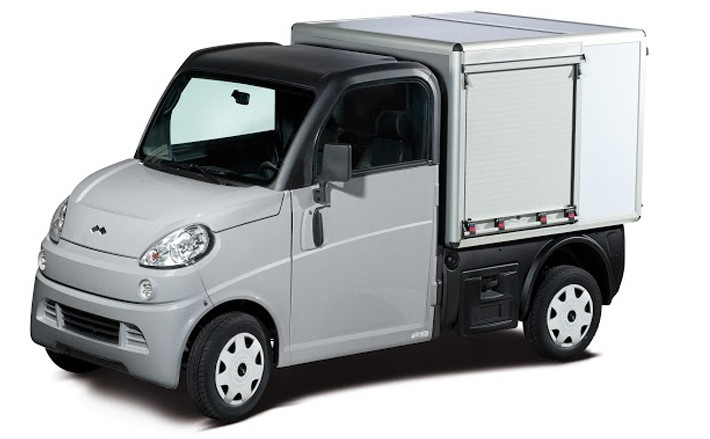
\includegraphics[width=0.8\textwidth]{furgon.jpg}
    \caption{Microcar Flex Furgon}
    \label{fig:furgon}
    % \vspace{0.5cm}
\end{figure}

\section{Powstawanie projektu}

\subsection{Hello World}
\begin{cppcode}
#include "Window.h"

Window::Window()
{
	width = 800;
	height = 600;
	xChange = 0;
	yChange = 0;
	mouseFirstMoved = true;
	for (size_t i = 0; i < 1024; i++) keys[i] = false;
}

Window::Window(GLint windowWidth, GLint windowHeight)
{
	width = windowWidth;
	height = windowHeight;
	xChange = 0;
	yChange = 0;
	mouseFirstMoved = true;
	for (size_t i = 0; i < 1024; i++) keys[i] = false;
}

int Window::Initialize()
{
	if (!glfwInit())
	{
		printf("Error Initialising GLFW");
		glfwTerminate();
		return 1;
	}

	glfwWindowHint(GLFW_CONTEXT_VERSION_MAJOR, 3);
	glfwWindowHint(GLFW_CONTEXT_VERSION_MINOR, 3);
	glfwWindowHint(GLFW_OPENGL_PROFILE, GLFW_OPENGL_CORE_PROFILE);
	glfwWindowHint(GLFW_OPENGL_FORWARD_COMPAT, GL_TRUE);
	glfwWindowHint(GLFW_REFRESH_RATE, 60);

	const GLFWvidmode* mode = glfwGetVideoMode(glfwGetPrimaryMonitor());
	mainWindow = glfwCreateWindow(width, height, "Microcar Flex Furgon", NULL, NULL);
	width = mode->width;
	height = mode->height;
	if (!mainWindow)
	{
		printf("Error creating GLFW window!");
		glfwTerminate();
		return 1;
	}

	glfwGetFramebufferSize(mainWindow, &bufferWidth, &bufferHeight);
	glfwMakeContextCurrent(mainWindow);
	createCallbacks();
	glfwSetInputMode(mainWindow, GLFW_CURSOR, GLFW_CURSOR_DISABLED);

	glewExperimental = GL_TRUE;

	GLenum error = glewInit();
	if (error != GLEW_OK)
	{
		printf("Error: %s", glewGetErrorString(error));
		glfwDestroyWindow(mainWindow);
		glfwTerminate();
		return 1;
	}

	glEnable(GL_DEPTH_TEST);
	glViewport(0, 0, bufferWidth, bufferHeight);
	glfwSetWindowUserPointer(mainWindow, this);
}

void Window::createCallbacks()
{
	glfwSetKeyCallback(mainWindow, handleKeys);
	glfwSetCursorPosCallback(mainWindow, handleMouse);
}

GLfloat Window::getXChange()
{
	GLfloat theChange = xChange;
	xChange = 0.0f;
	return theChange;
}

GLfloat Window::getYChange()
{
	GLfloat theChange = yChange;
	yChange = 0.0f;
	return theChange;
}

void Window::handleKeys(GLFWwindow* window, int key, int code, int action, int mode)
{
	Window* theWindow = static_cast<Window*>(glfwGetWindowUserPointer(window));

	if (key == GLFW_KEY_ESCAPE && action == GLFW_PRESS)
	{
		glfwSetWindowShouldClose(window, GL_TRUE);
	}
	else if (key >= 0 && key < 1024)
	{
		if (key == GLFW_KEY_B && action == GLFW_PRESS)
		{
			theWindow->keys[key] = !theWindow->keys[key];
		}
		else if (key == GLFW_KEY_B && action == GLFW_RELEASE)
			return;
		else if (action == GLFW_PRESS)
		{
			theWindow->keys[key] = true;
		}
		else if (action == GLFW_RELEASE)
		{
			theWindow->keys[key] = false;
		}
	}
}

void Window::handleMouse(GLFWwindow* window, double xPos, double yPos)
{
	Window* theWindow = static_cast<Window*>(glfwGetWindowUserPointer(window));

	if (theWindow->mouseFirstMoved)
	{
		theWindow->lastX = xPos;
		theWindow->lastY = yPos;
		theWindow->mouseFirstMoved = false;
	}

	theWindow->xChange = xPos - theWindow->lastX;
	theWindow->yChange = theWindow->lastY - yPos;

	theWindow->lastX = xPos;
	theWindow->lastY = yPos;
}

Window::~Window()
{
	glfwDestroyWindow(mainWindow);
	glfwTerminate();
}
\end{cppcode}

\begin{cppcode}
#pragma once

#include <stdio.h>
#include <string.h>
#include <math.h>
#include <vector>
#include <sstream>
#include <GL\glew.h>
#include "Window.h"

GLfloat deltaTime = 0.0f;
GLfloat lastTime = 0.0f;
GLfloat timeCounter = 0.0f;
int frameCount = 0;

static const char* vShader = "Shaders/shader.vert";
static const char* fShader = "Shaders/shader.frag";

void computeFPS(GLFWwindow* pWindow)
{
	GLfloat now = glfwGetTime();
	deltaTime = now - lastTime;
	lastTime = now;
	timeCounter += deltaTime;
	frameCount++;

	if (timeCounter >= 1.0) {
		double fps = double(frameCount) / timeCounter;

		std::stringstream ss;
		ss << " [" << fps << " FPS]";

		glfwSetWindowTitle(pWindow, ss.str().c_str());

		frameCount = 0;
		timeCounter = 0;
	}
}

int main()
{
	Window mainWindow(1200, 800);
	mainWindow.Initialize();

	while (!mainWindow.getShouldClose())
	{
		computeFPS(mainWindow.mainWindow);

		glfwPollEvents();

		glClearColor(0.0f, 0.0f, 0.0f, 1.0f);
		glClear(GL_COLOR_BUFFER_BIT | GL_DEPTH_BUFFER_BIT);

		glUseProgram(0);
		mainWindow.swapBuffers();
	}

	return 0;
}
\end{cppcode}


\subsection{Utworzenie podłoża}

\subsection{Stworzenie modeli 3D}

\begin{figure}[H]
    \centering
    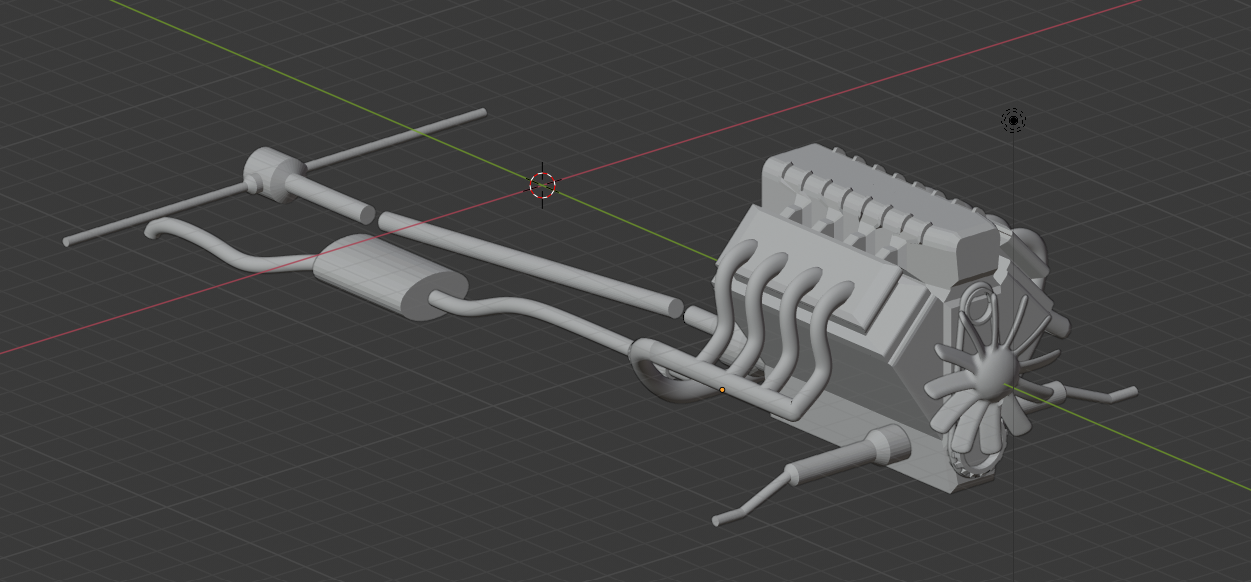
\includegraphics[width=\textwidth]{podwozie.png}
    \caption{Podwozie samochodu}
    \label{fig:podwozie}
    % \vspace{0.5cm}
\end{figure}


\subsection{Implementacja modeli w programie}
\subsection{Ożywienie samochodu}

\section{Podsumowanie}
\begin{figure}[h!]
    \centering
    \subfloat{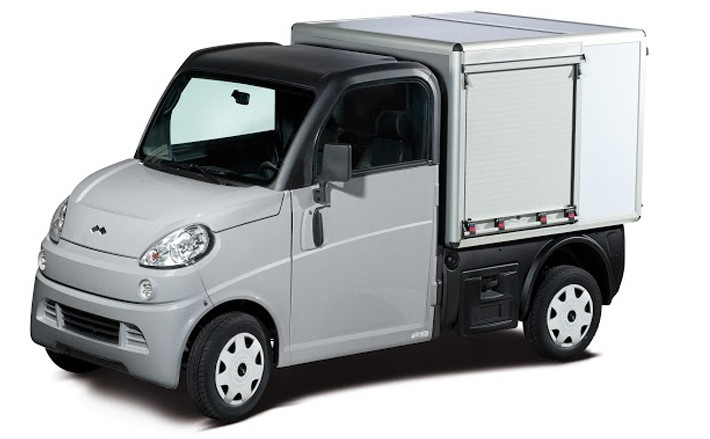
\includegraphics[width=0.5\textwidth]{furgon.jpg}}
    \subfloat{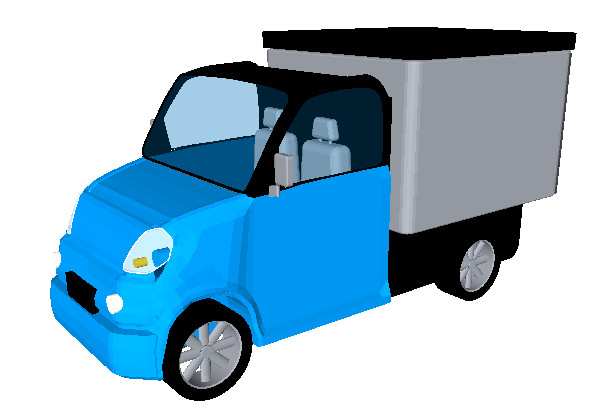
\includegraphics[width=0.5\textwidth]{gl_microcar.jpg}}
    \caption{Porównanie oryginału z utworzonym modelem}
    \label{fig:furgon}
    % \vspace{0.5cm}
\end{figure}

% \begin{pythoncode}
% def forward(self, x):
%     y, sum_inputs = [x], []
%     for i in range(len(self.layers) + 1):
%         f = self.linear if i == len(self.layers) else self.activation
%         s = [np.dot(y[i], w) for w in self.weights[i]] + self.biases[i]
%         y.append(f(s))
%         sum_inputs.append(s)
%     return y, sum_inputs
% \end{pythoncode}


% \pagebreak
\begin{thebibliography}{9}
    \addcontentsline{toc}{section}{Literatura}
    \bibitem{zajdel_9} T. Gałaj, \emph{Learn OpenGL}, \href{https://shot511.github.io/pages/learnopengl/}{https://shot511.github.io/pages/learnopengl/}
\end{thebibliography}

\end{document}